\subsection{Neural Networks}\label{neuralnet}
Neural Networks are a part of neurocomputing, which aims to develop computational systems inspired by the human brain's structure and function. For example, pattern recognition, motor control, vision, flexible inference, intuition, and accurate guessing are all skills the brain is particularly adept at, which is what neural networks aim to emulate \autocite{anderson1995introduction}. 

At a high level, a neural network is a collection of related nodes (called "neurons") arranged in layers. Data is sent to the input layer, where one or more hidden levels process it before being output by the final layer.

The basic unit of a neural network is a neuron, which receives input from other neurons or the input layer. The neuron then uses a mathematical function to this input, producing an output which is sent to other neurons in the next layer. The most commonly used function is the sigmoid function, given in \cref{eq:sigmoid}. 

\begin{equation}
    \sigma(z) = \frac{1}{1+e^{-z}}
    \label{eq:sigmoid}
\end{equation}

where $z$ is the input to the neuron. The sigmoid function always outputs a decimal between 0 and 1, which can be interpreted as a probability.

The output of a neuron is determined by the weights and biases associated with its inputs. Each input is multiplied by a weight, and these weighted inputs are summed together with a bias to produce the neuron's input, as shown in \cref{eq:z}. 

\begin{equation}
    z = \sum_{i=1}^n w_i x_i + b
    \label{eq:z}
\end{equation}

where $w_i$ is the weight, $x_i$ is the value of the $i$th input, $n$ is the number of inputs, and $b$ is the bias. 

\Cref{eq:y} exhibits the neuron output when applying the sigmoid function to the input.

\begin{equation}
    y = \sigma(z)
    \label{eq:y}
\end{equation}

During the training process, which includes feeding training data through the network (illustrated in \cref{fig:nn}) and modifying the weights and biases based on the difference between the predicted output and the actual output (target), the weights and biases of a neural network are adjusted. Usually, a gradient descent optimisation technique is used to carry out this operation.

\begin{figure}[h]
\resizebox{\textwidth}{!}{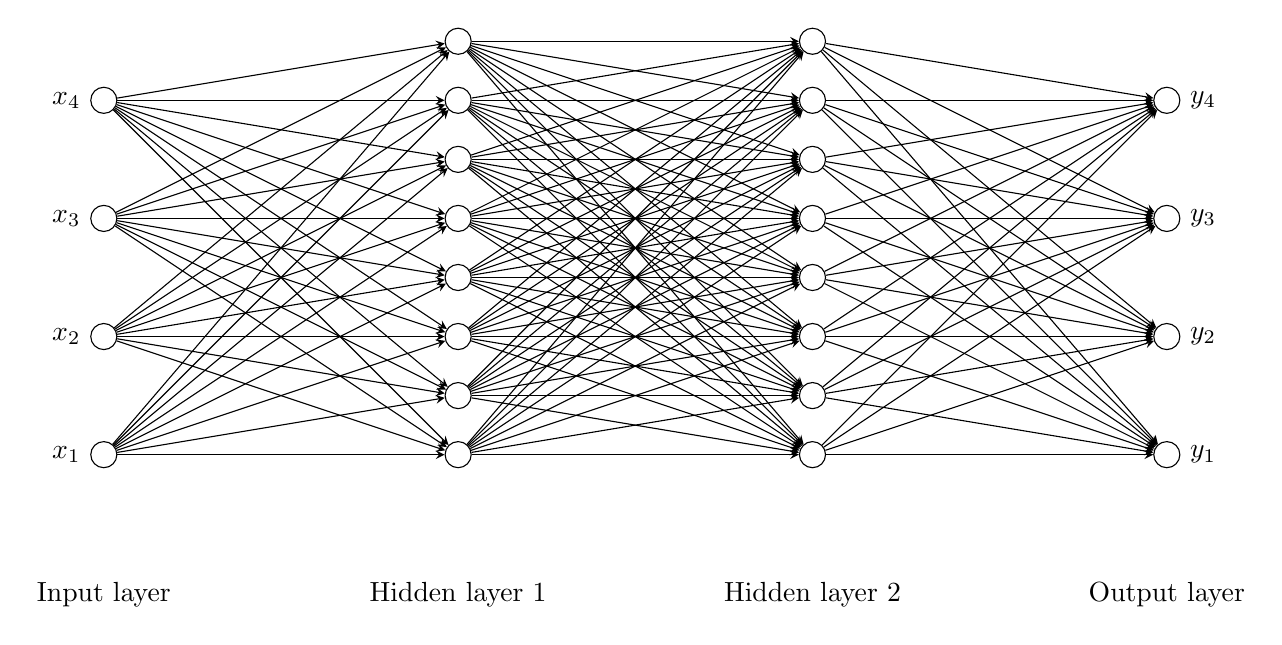
\begin{tikzpicture}[x=3cm, y=1.5cm, >=stealth]
    
    % Input layer nodes
    \foreach \i in {1,...,4} {
        \node[draw, circle] (input-\i) at (0, \i) {};
    }
    
    % First hidden layer nodes
    \foreach \i in {1,...,8} {
        \node[draw, circle] (hidden1-\i) at (1.5, 0.5 + 0.5*\i) {};
    }
    
    % Second hidden layer nodes
    \foreach \i in {1,...,8} {
        \node[draw, circle] (hidden2-\i) at (3, 0.5 + 0.5*\i) {};
    }
    
    % Output nodes
    \foreach \i in {1,...,4} {
        \node[draw, circle] (output-\i) at (4.5, \i) {};
    }

    % Input layer labels
    \foreach \i in {1,...,4} {
        \node[left] at (input-\i.west) {$x_{\i}$};
    }
    
    % Output layer labels
    \foreach \i in {1,...,4} {
        \node[right] at (output-\i.east) {$y_{\i}$};
    }
    
    % Connect input to first hidden layer
    \foreach \i in {1,...,4} {
        \foreach \j in {1,...,8} {
            \draw[->] (input-\i) -- (hidden1-\j);
        }
    }
    
    % Connect first hidden layer to second hidden layer
    \foreach \i in {1,...,8} {
        \foreach \j in {1,...,8} {
            \draw[->] (hidden1-\i) -- (hidden2-\j);
        }
    }
    
    % Connect second hidden layer to output
    \foreach \i in {1,...,8} {
        \foreach \j in {1,...,4} {
            \draw[->] (hidden2-\i) -- (output-\j);
        }
    }
    
    % Layer labels
    \node[below] at (0, 0) {Input layer};
    \node[below] at (1.5, 0) {Hidden layer 1};
    \node[below] at (3, 0) {Hidden layer 2};
    \node[below] at (4.5, 0) {Output layer};

\end{tikzpicture}}
\caption{Illustration of Neural Network}
\label{fig:nn}
\end{figure}